
        \documentclass[12pt]{article}
        \usepackage{bfcours}
        \usepackage[utf8]{inputenc}
        \usepackage{datatool}
        \usepackage{geometry}
        \usepackage{pgfplots}
        \pgfplotsset{compat=1.18}
        \usepgfplotslibrary{polar}
        \usepackage{pgfplotstable}
        \usepackage{float}
        \usepackage{multicol}
        \usepackage[most]{tcolorbox}
        \geometry{left=1cm,right=1cm,top=2cm,bottom=2cm}
        \usepackage{hyperref}

        \DTLsetseparator{;} % Assurez-vous que cela correspond au séparateur de votre fichier CSV.
        \usepackage{siunitx}
        \sisetup{output-decimal-marker={,}}
        \newcommand\boitesignature[2]{
        \begin{multicols}{2}
            \begin{tcolorbox}[nobeforeafter,colframe=white, % Couleur de la bordure
            colback=white, % Couleur de fond
            boxsep=0pt, % Pas d'espace entre le texte et les bords de la boîte
            top=0pt, bottom=0pt, left=0pt, right=0pt, % Pas de marges intérieures
            boxrule=0pt, % Pas de bordure visible
            height=3cm,
            arc=0pt, % Coins non arrondis
            ]
                #1
            \end{tcolorbox}
            
            \columnbreak
            
            \begin{tcolorbox}[nobeforeafter,height=3cm,title=\bfseries Résultat obtenu au contrôle :,halign title=flush left,fonttitle=\bfseries,colbacktitle=black,coltitle=white,colback=white]%red!50!black
                #2
            \end{tcolorbox}
        \end{multicols}
        }
        \begin{document}
            
\section{Résultats de LITTLEWOOD Boumbazar}

    %%% debut - tableau %%%
    \boitesignature{
    \textbf{Titre : }{''}
    \textbf{Contrôle effectué le : 04/05/2024} \\
    \textbf{Thèmes abordés : }
    }{\begin{center}\bfseries\huge{4/6} \end{center}}

    \begin{center}
        
\begin{tcbtab}[Par exercice :]{|c|c|c|c|}
      \hline
       & \bfseries Exercice 1  & \bfseries Exercice 2  & \bfseries Exercice 3  \\
      \hline
      \bfseries Points  & 2 & 0 & 2 \\
      \hline
      \bfseries Barème  & 1 & 3 & 2 \\
      \hline
\end{tcbtab}

    \end{center}

    %%% fin - tableau %%%

\begin{multicols}{2}

    %%% debut - explications %%%
    \boite{Commentaires :}{
        
            \begin{itemize}

                \item \textbf{Exercice 2} à retravailler.
            
            \end{itemize}

    
    }
    %%% fin - explications %%%
    
    \columnbreak

    %%% debut - radar %%%
    
    
\begin{center}
    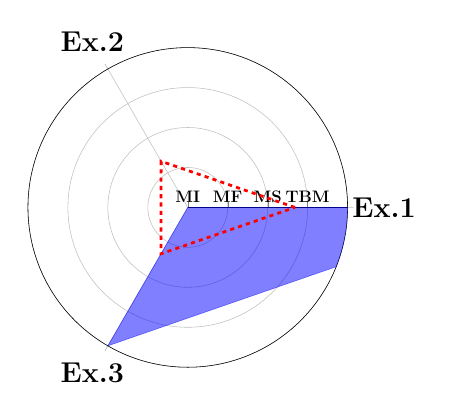
\begin{tikzpicture}[scale=0.5]
        \begin{polaraxis}[
            width=0.8\textwidth,
            xtick={0.0,120.0,240.0},
            xticklabels={\huge \bfseries Ex.1,\huge \bfseries Ex.2,\huge \bfseries Ex.3},
            ymin=0, ymax=100,
            ytick={0,25,50,75,100},
            yticklabels={\large \bfseries MI,\large \bfseries MF,\large \bfseries MS,\large \bfseries TBM, }
        ]
        \addplot+[mark=none,fill=blue,opacity=0.5] coordinates {
            (0.0,200.0)  (120.0,0.0)  (240.0,100.0)  
        } -- cycle;
        
        \addplot+[mark=none,fill=none,opacity=1,line width = 2pt,dashed,color=red] coordinates {
                    (0.0,67.0)  (120.0,33.333333333333336)  (240.0,33.5)  
                } -- cycle;
        
        \end{polaraxis}
    \end{tikzpicture}
\end{center}


    %%% fin - radar %%%

\end{multicols}

        \end{document}
        